%!TEX TS-program = xelatex
\documentclass[]{friggeri-cv}

\usepackage{afterpage}
\usepackage{hyperref}
\usepackage{color}
\usepackage{xcolor}
\definecolor{myblue}{RGB}{4, 98, 249}
\usepackage{hyperref}
\hypersetup{
    pdftitle={},
    pdfauthor={},
    pdfsubject={},
    pdfkeywords={},
    colorlinks=true,       % no lik border color
    allbordercolors=white    % white border color for all
}
%\addbibresource{bibliography.bib}
\RequirePackage{xcolor}
\definecolor{pblue}{HTML}{0395DE}


% ------------
\usepackage{enumitem}
\renewenvironment{entrylist}{%
  \begin{itemize}[leftmargin=1in]%[leftmargin=*,align=left,itemindent=-\dimexpr\labelwidth+\labelindent+\labelsep\relax]
  }{%
  \end{itemize}
}
\renewcommand{\bfseries}{\headingfont\color{headercolor}}
\renewcommand{\entry}[4]{%
\item[#1]
  \textbf{#2}%
  \hfill%
  {\footnotesize\addfontfeature{Color=myblue} #3}\\%
  #4\vspace{\parsep}%
}
% -------


\begin{document}
\header{Boyang}{Yan}
     
% Fake text to add separator      
\fcolorbox{white}{gray}{\parbox{\dimexpr\textwidth-2\fboxsep-2\fboxrule}{%
.....
}}

% In the aside, each new line forces a line break
\begin{aside}
  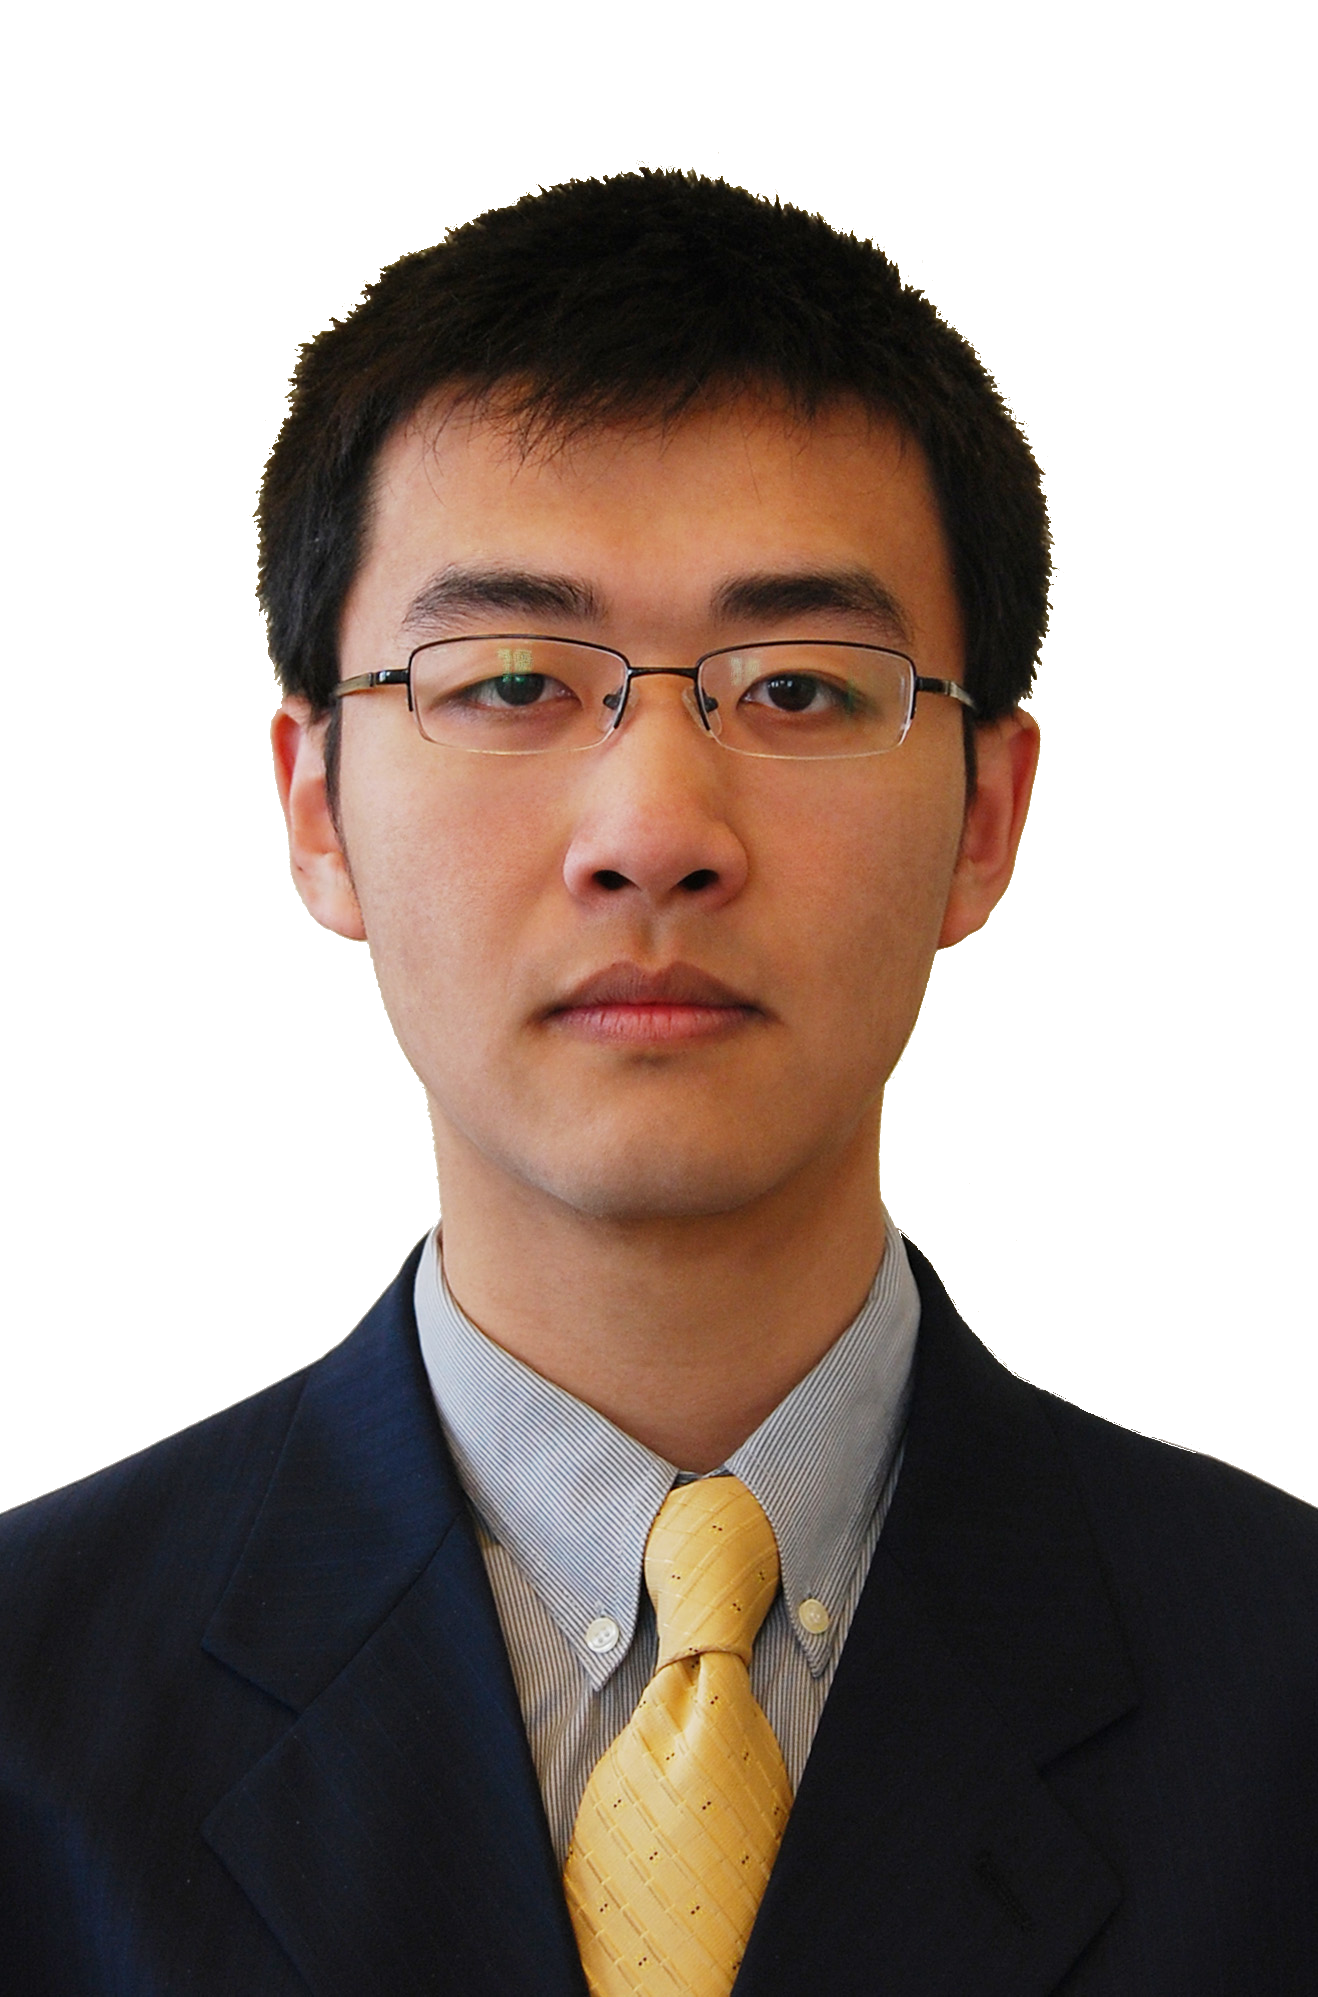
\includegraphics[scale=0.007]{img/boyang.png}
  \section{Address}
  14-6-602 Zhuhuali Community, Huayuanxincheng
  Nankai District,  Tianjin,
  China
    ~
  \section{Contact Info}
  \textbf{Tel:} +86 18512290791
    \textbf{Wechat:} yanboyang713
    ~
  \section{Mail}
  \href{mailto:yanboyang713@gmail.com}{\textbf{yanboyang713@}\\gmail.com}
    \href{mailto:boyangy3@illinois.edu}{\textbf{boyangy3@}\\illinois.edu}
    ~
  \section{Web \& Git}
    \href{https://github.com/yanboyang713}{github.com/yanboyang713}
    \href{https://www.researchgate.net/profile/Boyang_Yan}{researchgate.net}
    ~
  \section{Programming}
    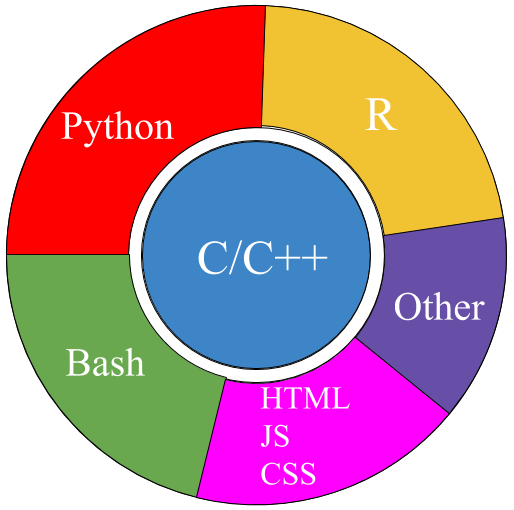
\includegraphics[scale=0.2]{img/programming.png}
    ~
  \section{OS Preference}
    \textbf{GNU/Linux}
\includegraphics[scale=0.40]{img/5stars.png}
    \textbf{Unix}
\includegraphics[scale=0.40]{img/4stars.png}
    \textbf{MacOS}
\includegraphics[scale=0.40]{img/3stars.png}
    \textbf{Windows}
\includegraphics[scale=0.40]{img/1stars.png}
    ~
\end{aside}

\section{Personal Evaluation}
I see myself advancing with a strong ability and interesting in new technology
and academic research.
I successfully participated two international academic conferences,
one published paper and one patent. In the University study, I got undergraduate
scholarships and the best prize for final project. The final project is related
to swipe card system. I would like the chance to take specific field of Computer
Science to prepare myself for other roles in the Domain. I want to build my new
academic experience with UVIC education and training.

\section{Working Experience}
\begin{entrylist}
  \entry
  {2020.3 - now\\}
  {\large{Support Engineer}\\}
  {Microsoft, China}
  {Azure Machine Learning CSS Team}

  \entry
  {2018.12 - 2020.3\\}
  {\large{Algorithm Engineer}\\}
  {Peng Chen Laboratory, China}
  {Network Communication Research Center}

\entry
{2018.1 - 2018.11\\}
{\large{Research Assistant} (Computer Science)\\}
{University of Wollongong, Australia}
{Metamorphic Testing - Software Testing}

\end{entrylist}

\section{Education}
\begin{entrylist}
  \entry
  {2019.3 - now\\}
  {\large{Netmath}​}
  {University of Illinois (Urbana–Champaign)}
  {Major in Mathematics\\
    \textbf{Main subjects}:\\
    Algebra A+\\
    Preparation for Calculus A+
  }

  \entry
    {2014.3 - 2017.12\\}
    {\large{Bachelor of Computer Science}​}
    {University of Wollongong, Australia}
    {Major in Software Engineering\\
      \textbf{Main subjects}:\\
      Algorithms and Data Structures(80 Distinction)\\
      Object and Generic Programming in C++ (75 Distinction)\\
      Interactive Computer Graphics (75 Distinction)\\
      Multimedia Computing (73 Credit)\\
      software Engineering Practices \& Principles (82 Distinction)\\
      \textbf{Main Achievement}:\\
      1. The best final project prize ({\footnotesize Human Research Management System base on Web})\\
      2. First Three Semester had: Undergraduate Excellence Scholarship\\
    }
  \entry
  {2013.3 - 2014.3}
  {\large{English for Tertiary Studies}}
  {University of Wollongong College, Australia}
  {Main subjects: Academic English}

  \entry
    {2011.9 - 2013.3\\}
    {\large{Bachelor of Business Management}\\}
    {China University Of Mining And Technology}
    {Average mark of 91\% . Most of courses got High Distinction}

  \end{entrylist}

\newpage

\section{Publications}
Boyang Yan, Brian Yecies, Zhi Quan Zhou: Metamorphic Relations for Data
Validation: A Case Study of Translated Text Messages. IEEE/ACM 4th International
Workshop on Metamorphic Testing (MET '19), in conjunction with the 41st
International Conference on Software Engineering (ICSE '19), Montreal, Canada;
05/2019

\section{Patents}

\begin{entrylist}
  \entry
  {June 2, 2020}
  {An automated text difference analysis and verification system/method}
  {China Patent Office Application ID: 202010489931.8}

\end{entrylist}


\section{Academy Congress and Conference}
\begin{entrylist}
  \entry
  {May 26, 2019}
  {\\Paper Presentation - Title: Metamorphic Relations for Data Validation: A Case Study of Translated Text Messages}
  {ICSE, Montreal, Canada}

  \entry
  {August 11, 2017}
  {showing my final year project about Human Resource Management System based on
    Web (whole swap card subsystem and database are finish independently)\\}
  {IEEE Sections Congress (SC2017), Sydney, Australia}

\end{entrylist}

\section{Certifications}
\begin{entrylist}
  \entry
  {2019}
  {First Aid CPR AED\\}
  {American Heart Association}


  \entry
    {2017}
    {Amateur Radio Operator's certificate of proficiency (Standard)\\}
    {The Wireless Institute of Australia (WIA)}

  \entry
    {2016}
    {Ross a. Hull memorial Vhf-Uhf contest\\}
    {The Wireless Institute of Australia (WIA)}
    {Twelfth Place in Section A (Analog Modes, Best
7 Days) and Twelfth Place in Section C (Analog Modes, Best 2 Days)}

  \entry
    {2014}
    {Amateur Radio Operator's certificate of proficiency (Foundation)\\}
    {The Wireless Institute of Australia (WIA)}
   
  \entry
    {2010}
    {The Second Place Prize Awarded, Tianjin School Sports Competition Award "92" National Games Tianjin\\}
    {Tianjin Basketball Tryouts, China}
    {High school men's Group B. Primary and Secondary (Vocational) School Basketball Games. Have got the second grading certificate and title}

  \end{entrylist}

\begin{aside}
  \section{Languages}
    \textbf{Chinese}
\includegraphics[scale=0.40]{img/5stars.png}
    \textbf{English}
\includegraphics[scale=0.40]{img/4stars.png}
\end{aside}

%%% This piece of code has been commented by Karol Kozioł due to biblatex errors. 
% 
%\printbibsection{article}{article in peer-reviewed journal}
%\begin{refsection}
%  \nocite{*}
%  \printbibliography[sorting=chronological, type=inproceedings, title={international peer-reviewed conferences/proceedings}, notkeyword={france}, heading=subbibliography]
%\end{refsection}
%\begin{refsection}
%  \nocite{*}
%  \printbibliography[sorting=chronological, type=inproceedings, title={local peer-reviewed conferences/proceedings}, keyword={france}, heading=subbibliography]
%\end{refsection}
%\printbibsection{misc}{other publications}
%\printbibsection{report}{research reports}

\end{document}
